\documentclass[11pt]{article}
\usepackage[margin=1in]{geometry}
\usepackage{amsmath,amssymb,amsthm}
\usepackage{graphicx}
\usepackage{booktabs}
\usepackage{hyperref}
\usepackage{natbib}
\usepackage{xcolor}
\usepackage{microtype}
\usepackage{algorithm}
\usepackage{algpseudocode}

\newcommand{\Gr}{\mathrm{Gr}}
\newcommand{\BN}{\mathrm{BN}}
\newcommand{\R}{\mathbb{R}}
\newcommand{\TODO}[1]{\textcolor{red}{[TODO: #1]}}
\newcommand{\CITE}[1]{\textcolor{red}{[CITE: #1]}}

\title{Geometric and Causal Audit of RNA Foundation Model Representations:\\
  Transportability Collapse, Linear Repeat-Count Encoding, and\\
  Cross-Disease Universality on Polyglutamine mRNAs}

\author{Elliot Tower\\
  Mechanistic Research\\
  \texttt{elliot@elliottower.ai}}

\date{July 2026}

\begin{document}
\maketitle

\begin{abstract}
RNA foundation models are increasingly proposed for therapeutic target
identification, yet the geometric and causal validity of their
representations remains untested on disease-relevant sequences. We
apply twelve independent audits to RNA-FM (99M parameters) on
polyglutamine-disease mRNAs, combining geometric analysis with causal
probing under a preregistered protocol with SHA-frozen scorer code.

Six geometric audits on HTT mRNA CAG repeat variants establish three
findings. RNA-FM's learned representations and ViennaRNA thermodynamic
structure predictions are statistically independent ($|r| < 0.09$,
Grassmannian overlap indistinguishable from shuffled controls).
Embedding subspaces undergo near-complete rotation ($d_g \approx 3.7$,
principal angles $> 85^\circ$) for any change in repeat count, with no
phase transition at the disease threshold. Direction instability loses
resolution on rank-1-collapsed layers (uniform to six decimal places at
layer~6), recovering genuine signal only at high-dimensionality layers.

Six causal probes reveal a paradoxical encoding. Distributed Alignment
Search finds a single linear direction encoding CAG repeat count at
layer~0 with $R^2 = 0.992$ ($n = 71$ variants), yet this information
is progressively destroyed through the network. By the output layer,
repeat count has zero effect on predictions (100\% top-1 MLM agreement,
KL divergence $\sim 10^{-6}$). A CAA synonym control ($R^2 = 0.993$)
shows the encoding is structure-agnostic --- the model counts
trinucleotide repetitions regardless of RNA hairpin formation.
Replication across all six human polyglutamine disease genes (HTT,
ATXN1, ATXN2, ATXN3, AR, ATN1; all $R^2 > 0.98$) confirms
universality, while cross-gene direction cosine analysis reveals two
encoding clusters (mean $|\cos| = 0.73$): HTT diverges from the other
five genes, which share a common encoding subspace ($|\cos| = 0.80$--$0.88$).
EAP-IG circuit attribution shows information destruction is
MLP-dominated (79\% of attribution), concentrated in late layers.

The model represents the clinically relevant variable with high
fidelity but does not compute with it. All code, data, and
preregistration records are publicly available.
\end{abstract}

%% ────────────────────────────────────────────
\section{Introduction}
\label{sec:intro}

Huntington's disease (HD) is caused by expansion of a CAG trinucleotide
repeat in exon~1 of the Huntingtin gene (HTT), producing a
polyglutamine-expanded protein that aggregates and causes
neurodegeneration~\citep{macdonald1993}.
Normal alleles carry 6--35 CAG repeats; 36--39 repeats confer incomplete
penetrance; 40+ repeats are fully penetrant~\citep{rubinsztein1996}.
No disease-modifying therapy exists. The primary therapeutic strategy
targets HTT mRNA directly, using antisense oligonucleotides (ASOs) to
reduce production of the toxic protein~\citep{tabrizi2019}.

The central challenge for RNA-targeting drug design is \emph{transportability}:
a drug mechanism validated on one CAG repeat length must transfer to the
repeat lengths seen in patients. Clinical trials of tominersen
(an ASO targeting HTT mRNA) were halted partly because the drug reduced
both mutant and wild-type HTT with insufficient selectivity~\citep{tabrizi2022}.
Understanding which structural features of the CAG repeat region are
preserved across repeat lengths---and which degrade---would inform
the design of allele-selective therapies.

RNA foundation models offer a new lens on this problem. RNA-FM, a
99M-parameter BERT-style model pre-trained on 23 million non-coding RNA
sequences, produces 640-dimensional contextual embeddings for each
nucleotide position~\citep{rnafm}. These embeddings
capture structural and functional properties learned from evolutionary
data, providing a representation space where geometric analyses can
detect genuine structural signals --- or reveal their absence.

We apply twelve complementary audits from the causal geometry
framework~\citep{tower2026bn,tower2026grass}
to RNA-FM embeddings of CAG repeat regions across all six human
polyglutamine disease genes, under a preregistered analysis protocol
with SHA-frozen scorer code. The audits fall into two groups.

\paragraph{Geometric audits (HTT).}
\begin{enumerate}
\item \textbf{Bracket-norm correction.} The bracket
  norm~\citep{tower2026bn} normalizes feature magnitudes by $\sqrt{n}$
  to distinguish \emph{intensive} structural properties (genuine
  features of the RNA fold) from \emph{extensive} properties (artifacts
  scaling with input length).

\item \textbf{Grassmannian transportability.} For each CAG repeat count
  $r$, PCA of the embedding region yields a point on the Grassmannian
  $\Gr(k, 640)$. Geodesic distance from the wild-type subspace
  quantifies drug mechanism
  transferability~\citep{tower2026grass}.

\item \textbf{Weight factorization.} SVD of RNA-FM's attention and MLP
  weight matrices reveals intrinsic dimensionality and cross-projection
  subspace overlap, testing whether the model admits a shared factor
  bank decomposition~\citep{tower2026fac}.

\item \textbf{Direction instability (DI).} Per-position cosine
  dissimilarity between wild-type and mutant embeddings, measured as
  $\mathrm{DI} = 1 - \bar{c}$ where $\bar{c}$ is the mean pairwise
  cosine similarity across variants.

\item \textbf{Cross-view thermodynamic validation.} ViennaRNA
  base-pair probabilities~\citep{lorenz2011viennarna} provide a
  physics-based structural view independent of the learned model.

\item \textbf{Layer-resolved metric sensitivity.} Effective
  dimensionality (95\% PCA variance threshold) across layers identifies
  where rank-1 collapse renders directional metrics uninformative.
\end{enumerate}

\paragraph{Causal probes (six polyglutamine genes).}
\begin{enumerate}
\setcounter{enumi}{6}
\item \textbf{Distributed Alignment Search (DAS).} A learned orthogonal
  rotation projects the 640-dimensional hidden state onto $k$ dimensions
  trained to predict repeat count via MSE loss. Layer-by-layer $R^2$
  traces the encoding trajectory through the network.

\item \textbf{Behavioral invariance.} Masked-position predictions are
  compared across repeat-count variants at aligned flanking positions,
  testing whether encoded repeat-count information reaches the output.

\item \textbf{CAA synonym control.} CAA encodes the same amino acid
  (glutamine) as CAG but forms no RNA hairpin structure. Repeating DAS
  with CAA repeats tests whether the model encodes trinucleotide count
  or RNA secondary structure.

\item \textbf{Cross-disease universality.} Repeating the full DAS
  analysis on the five other human genes with pathogenic CAG repeat
  expansions (ATXN1, ATXN2, ATXN3, AR, ATN1) tests generality beyond
  a single gene.

\item \textbf{EAP-IG circuit attribution.} Edge Attribution Patching
  with Integrated Gradients decomposes the total attribution into
  per-head and per-MLP-layer contributions, identifying the computational
  circuit for CAG-region processing.

\item \textbf{Cross-gene direction cosine.} DAS directions learned
  independently for each gene are compared via pairwise $|\cos|$,
  testing whether the model uses a universal encoding direction or
  gene-specific ones.
\end{enumerate}

Together, the geometric audits establish validity constraints on
structural claims derived from RNA-FM embeddings, while the causal
probes characterize what the model actually encodes and computes.
The strongest combined result is the paradox between encoding fidelity
($R^2 = 0.992$) and behavioral inertness (KL $\sim 10^{-6}$): the
model represents repeat count with high precision but does not use it.


%% ────────────────────────────────────────────
\section{Background}
\label{sec:background}

\subsection{RNA-FM architecture}

RNA-FM~\citep{rnafm} is a BERT-style~\citep{devlin2019bert}
transformer encoder with 12 layers, 20 attention heads per layer,
hidden dimension $d = 640$, and intermediate MLP dimension $d_{\mathrm{ff}} = 5120$.
The model uses a nucleotide-level vocabulary of 28 tokens (A, C, G, U,
plus special tokens) and was pre-trained with masked language modeling
on 23.7 million non-coding RNA sequences from RNAcentral.
%
RNA-FM achieves state-of-the-art performance on RNA secondary structure
prediction, producing per-nucleotide embeddings that encode structural
context without explicit thermodynamic modeling.

\subsection{HTT mRNA and CAG repeat structure}

The human HTT mRNA (RefSeq NM\_002111.7) spans 13{,}669 nucleotides.
The pathogenic CAG repeat lies in exon~1, with normal alleles containing
approximately 21 repeats (63 nucleotides). The repeat region and its
flanking sequences create a structured RNA domain whose conformation
depends on repeat length: longer repeats form more stable hairpin
structures that may affect mRNA splicing, localization, and
translation~\citep{demezer2011,sobczak2003}.

\subsection{Bracket norm}

The bracket norm~\citep{tower2026bn} is a normalization that
distinguishes intensive from extensive properties in high-dimensional
feature spaces. For a feature vector $\mathbf{f} \in \R^d$ computed
from $n$ observations, the bracket-norm corrected value is
$\BN(\mathbf{f}) = \|\mathbf{f}\| / \sqrt{n}$.
%
Features whose bracket-norm corrected magnitude is invariant to $n$
represent genuine intensive properties; features whose corrected
magnitude varies with $n$ are extensive and may be confounded by
sampling density or input size. In the RNA context, $n$ is the
sequence length, and the correction identifies embedding dimensions
that encode per-nucleotide structural information rather than
global sequence statistics.

\subsection{Grassmannian subspace analysis}

A $k$-dimensional subspace of $\R^d$ is a point on the Grassmannian
manifold $\Gr(k, d)$~\citep{edelman1998}. Given two subspaces
$U, V \in \Gr(k, d)$, the principal angles
$\theta_1 \leq \cdots \leq \theta_k$ between them are computed via the
SVD of $U^\top V$, and the geodesic distance is
$d_g(U, V) = \sqrt{\sum_i \theta_i^2}$.
%
This distance quantifies structural similarity between representation
subspaces: small geodesic distance implies that the same geometric
features are active in both conditions, while large distance indicates
a qualitative shift in representation structure.
%
When applied to RNA embeddings across CAG repeat variants, this yields
a \emph{transportability score}: the degree to which drug-relevant
structural features identified on wild-type RNA persist in disease-length
expansions.


\subsection{Direction instability}

Direction instability (DI) measures how much a per-position embedding
direction shifts under sequence perturbation. For a set of $m$ sequence
variants with embeddings $\{\mathbf{h}_i^{(1)}, \ldots,
\mathbf{h}_i^{(m)}\}$ at position $i$, the DI at position $i$ is
\[
  \mathrm{DI}(i) = 1 - \frac{1}{\binom{m}{2}} \sum_{j < k}
  \frac{\mathbf{h}_i^{(j)} \cdot \mathbf{h}_i^{(k)}}
       {\|\mathbf{h}_i^{(j)}\| \, \|\mathbf{h}_i^{(k)}\|}.
\]
High DI indicates that the model's representation at position $i$ is
sensitive to the perturbation; low DI indicates directional stability.
The metric ranges from 0 (identical directions) to 2 (antipodal).

DI is a directional metric: it measures angles between embedding
vectors, ignoring magnitudes. On a layer where representations have
collapsed to near-rank-1 (a single dominant principal component), all
positions share approximately the same direction, so DI becomes
uninformative. The metric's resolution therefore depends on the
effective dimensionality of the representation.

\subsection{Cross-view validation}

A cross-view analysis tests whether two independent measurement
modalities recover the same structural features. We treat RNA-FM
embeddings and ViennaRNA minimum free energy (MFE) base-pair
probabilities~\citep{lorenz2011viennarna} as two views of the same
RNA sequence. If the learned model has captured thermodynamic
structure, its principal component subspace should overlap with the
subspace spanned by physics-based structural features. Independence
between the two views indicates that RNA-FM encodes features
orthogonal to classical RNA secondary structure.


%% ────────────────────────────────────────────
\section{Methods}
\label{sec:methods}

\subsection{Data preparation}

We obtained the full-length HTT mRNA sequence (NM\_002111.7,
13{,}669~nt) from NCBI RefSeq. The native CAG repeat region was
identified by regex matching, yielding 21 tandem CAG repeats at
positions 148--211.

To study transportability across repeat lengths, we constructed
synthetic HTT mRNA variants by replacing the native CAG repeat with
$r \in \{15, 21, 27, 36, 40, 50, 60, 80\}$ tandem repeats, preserving
50~nt of flanking sequence on each side. This set spans
sub-normal (15), normal (21), intermediate (27), reduced-penetrance
threshold (36), full-penetrance (40), and severe expansion (50--80)
alleles.

\subsection{Embedding extraction}

We loaded RNA-FM weights from the HuggingFace
repository into a BERT encoder using the
\texttt{transformers} library~\citep{wolf2020transformers}, with
architecture parameters matched to the published
specification (12 layers, 640 hidden, 20 heads, 5120 intermediate).
%
Input sequences were tokenized at single-nucleotide resolution
(A$\to$5, C$\to$6, G$\to$7, U$\to$8) with CLS and EOS tokens.
Embeddings from the final hidden layer and all intermediate layers
were extracted for each variant.

\subsection{Bracket-norm analysis}

For windows of size $n \in \{100, 200, 300, 400, 500\}$~nt centered on
the CAG repeat region, we computed the mean embedding norm
$\bar{\ell}(n) = \frac{1}{n} \sum_{i=1}^{n} \|\mathbf{h}_i\|$
and the bracket-norm corrected value $\BN(n) = \bar{\ell}(n) / \sqrt{n}$.
%
An intensive property yields constant $\BN(n)$ across window sizes;
an extensive property yields $\BN(n)$ that decreases as $1/\sqrt{n}$.

We also computed per-dimension bracket norms: for each of the 640
embedding dimensions, we computed the $L^2$ norm across positions and
divided by $\sqrt{n}$, identifying the dimensions with the highest
intensive signal.

\subsection{Grassmannian transportability}

For each CAG repeat variant $r$, we computed RNA-FM embeddings on the
synthetic sequence and extracted the final-layer representations for
the repeat-plus-flanking region. PCA with $k = 10$ components yielded
a subspace $U_r \in \Gr(10, 640)$.

The geodesic distance $d_g(U_{21}, U_r)$ between the wild-type
subspace and each variant subspace quantifies transportability.
We also computed the full principal angle spectrum to identify which
subspace dimensions are preserved versus disrupted by repeat expansion.

\subsection{Layer-wise analysis}

For a 500~nt window centered on the CAG repeat, we extracted hidden
states from all 13 layers (embedding + 12 transformer layers) and
performed PCA on each. The effective dimensionality (number of
components for 95\% variance) characterizes how concentrated the
representation is at each processing stage.

We computed cross-layer subspace similarity as the mean cosine of
principal angles between 10-dimensional PCA subspaces of different
layers, yielding a $13 \times 13$ similarity matrix.

\subsection{Weight matrix factorization}

For each of the 12 transformer layers, we performed SVD on all six
projection matrices ($W_Q, W_K, W_V, W_O \in \R^{640 \times 640}$
and $W_{\mathrm{in}} \in \R^{5120 \times 640}$,
$W_{\mathrm{out}} \in \R^{640 \times 5120}$).
%
The effective rank at 95\% cumulative variance and the spectral decay
ratio $\sigma_1 / \sigma_{10}$ characterize the intrinsic
dimensionality of each projection.

To assess whether projections share a common factor structure, we
computed the subspace overlap between the top-20 right singular vectors
of each attention projection pair ($W_Q$--$W_K$, $W_Q$--$W_V$,
$W_K$--$W_V$, $W_Q$--$W_O$) within each layer. High overlap indicates
that the same input-space directions are important across projections,
supporting a shared factor bank decomposition.

\subsection{Direction instability analysis}

For each CAG repeat variant $r \in \{10, 15, 18, 21, 24, 27, 30, 36,
40, 50, 60, 80\}$, we constructed the full-length HTT mRNA with the
specified repeat count and extracted per-position embeddings at each
layer. Positions were aligned across variants using a codon-level
scheme: 50 flanking nucleotides on each side were aligned by absolute
position, and CAG codons were mean-pooled to a single vector per codon
(10 codons per variant after truncation to the shortest variant's
length), yielding a fixed-size position matrix per variant.

DI was computed against the wild-type ($r = 21$) reference as
$\mathrm{DI}_r(i) = 1 - \cos(\mathbf{h}_i^{(r)},
\mathbf{h}_i^{(21)})$. We tested whether DI at each position
correlates with repeat-count deviation $|r - 21|$ (Spearman $\rho$,
Bonferroni-corrected $\alpha = 0.0125$ for four confirmatory
hypotheses).

\subsection{Cross-view thermodynamic validation}

ViennaRNA~\citep{lorenz2011viennarna} base-pair probabilities were
computed for each variant using \texttt{RNAfold --MEA -p} on a 263~nt
window (100~nt flanking + CAG region + 100~nt flanking). Base-pair
probability at each position, summed over all pairing partners, yields
a per-position scalar $\mathrm{bp\_prob}(i) \in [0, 1]$
representing thermodynamic pairing propensity.

Cross-view analysis proceeded in two steps. First, PC-level
correlation: for each of the top-10 PCA components of the RNA-FM
embedding matrix, we computed $|r|$ (Pearson) between the component
scores and position-matched bp\_prob values. Second, subspace
geodesic: PCA scores for both modalities were QR-orthonormalized in
a shared position space, and the geodesic distance between the
resulting subspaces was compared to a null distribution from 100
randomly shuffled sequences of the same nucleotide composition.

\subsection{Layer-resolved controls}

The entire DI analysis was repeated at layer~1 (effective
dimensionality $\approx 51$) in addition to the preregistered
layer~6 (effective dimensionality $\approx 1$). A length-matched
control replaced CAG repeats with CAA repeats of identical count,
testing whether flanking-region DI--repeat-count correlations reflect
repeat-specific semantics or generic length sensitivity.

\subsection{Preregistration protocol}

All confirmatory hypotheses (H1, H2, H5, H6) and the analysis code
were frozen before data collection. The scorer script
(\texttt{direction\_instability.py}) was committed at SHA
\texttt{5427db9} and recorded in \texttt{PREREGISTRATION.md} with
timestamp. The Bonferroni-corrected significance threshold
$\alpha = 0.05 / 4 = 0.0125$ was specified in advance. Exploratory
analyses (H3, H4, H7) were labeled as such before execution.
Layer~6 was preregistered as the primary analysis layer; the layer~1
re-analysis was motivated by the rank-1 collapse discovered during
the preregistered run and is reported as a post-hoc control.


\subsection{Distributed Alignment Search}

Distributed Alignment Search (DAS)~\CITE{geiger2024das} learns an
orthogonal rotation $R \in \R^{d \times d}$ such that the first $k$
coordinates of $Rh$ predict a scalar variable of interest. For each
condition (gene $\times$ codon), we constructed $n = 71$ synthetic mRNA
variants ($r = 10$ to $r = 80$, step 1) with 50~nt flanking context on
each side. The mean hidden state across the repeat region was extracted
at each of the 13 layers.

DAS was trained via MSE loss on normalized repeat count (500 epochs,
Adam, lr $= 10^{-3}$, orthogonality regularization
$\lambda_{\mathrm{orth}} = 0.1$). After training, $R$ was
orthonormalized via QR decomposition. Encoding quality was measured by
Pearson $R^2$ and Spearman $\rho$ between the projected value and
true repeat count.

\subsection{Behavioral invariance}

To test whether encoded repeat-count information reaches the output, we
compared masked-position MLM predictions across repeat-count variants.
For 6 repeat-count pairs $\times$ 20 flanking positions (120
evaluations), we masked a single nucleotide and compared the
predicted probability distributions between the two repeat counts.
Top-1 agreement and KL divergence quantify behavioral sensitivity.

\subsection{CAA synonym control}

CAA encodes the same amino acid (glutamine) as CAG but does not form
the RNA hairpin secondary structure associated with pathogenic CAG
repeats~\citep{demezer2011}. We repeated the full DAS analysis with
CAA repeats in HTT flanking context, using identical data generation
and training. If $R^2_{\mathrm{CAA}} \approx R^2_{\mathrm{CAG}}$,
the model counts trinucleotide repetitions independent of secondary
structure.

\subsection{Cross-disease universality}

We obtained mRNA sequences for the five other human genes with
pathogenic CAG repeat expansions: ATXN1 (SCA1), ATXN2 (SCA2),
ATXN3 (SCA3/Machado-Joseph disease), AR (SBMA/Kennedy disease),
and ATN1 (DRPLA). For each gene, the CAG repeat region was identified
in the RefSeq mRNA (NM\_000332.4, NM\_002973.4, NM\_004993.6,
NM\_000044.6, NM\_001940.4), and synthetic variants were generated
as for HTT.

\subsection{EAP-IG circuit attribution}

Edge Attribution Patching with Integrated Gradients computes per-head
and per-MLP-layer gradient $\times$ activation attributions for the
CAG-processing circuit. At each layer, forward hooks capture attention
and MLP sublayer outputs; a KL-based metric between clean and corrupted
logits is backpropagated to compute attribution scores. The corrupted
input replaces the CAG repeat count with a different value while
holding flanking context constant. Attribution is reported per head
(reshaped from the hidden dimension to $n_{\mathrm{heads}} \times
d_{\mathrm{head}}$) and per MLP sublayer.

\subsection{Cross-gene direction cosine}

DAS was trained independently at layer~0 ($k = 1$) for each of
7 conditions (HTT-CAG, HTT-CAA, ATXN1, ATXN2, ATXN3, AR, ATN1).
The pairwise $|\cos|$ matrix of the 640-dimensional direction vectors
tests whether RNA-FM uses a single universal encoding direction or
condition-specific ones. The matrix was compared against two
hypotheses: universal encoding ($|\cos| \approx 1$ everywhere) and
gene-specific encoding ($|\cos| \approx 0$ between genes).


%% ────────────────────────────────────────────
\section{Results}
\label{sec:results}

\subsection{LayerNorm absorbs per-position magnitude variation}

The mean per-position embedding norm is $28.667 \pm 0.001$ across all
window sizes (100--500~nt), yielding a bracket-norm corrected value
that decreases monotonically as $1/\sqrt{n}$ (from 2.867 at $n=100$
to 1.282 at $n=500$). This constancy reflects the LayerNorm applied
at every transformer layer: magnitude information is normalized away,
and structural differences between nucleotide positions are encoded
entirely in the \emph{directions} of the embedding vectors.

Per-dimension bracket norms identify a sparse set of intensive
dimensions. The top 10 dimensions (indices 548, 527, 401, 590, 511,
1, 505, 287, 442, 124) carry bracket-norm corrected values of
$3.38$--$2.79$, while the median dimension has a corrected value of
$1.42$. These high-bracket-norm dimensions represent the directions
most likely to encode genuine per-nucleotide structural properties
rather than positional artifacts.

\begin{figure}[h]
\centering
\includegraphics[width=0.9\textwidth]{../figures/bracket_norm_per_dim.png}
\caption{Per-dimension bracket-norm corrected values for the 640
RNA-FM embedding dimensions on the HTT CAG region. The distribution
is right-skewed: a minority of dimensions carry disproportionately
high intensive signal. Dimensions above the median (dashed) are
candidates for structural feature extraction.}
\label{fig:bracket_norm}
\end{figure}

\subsection{Grassmannian transportability collapses for any repeat-count change}

The wild-type representation subspace ($r = 21$) is dominated by its
first principal component, which explains 95.7\% of variance. This
near-one-dimensional structure means the $k=10$ PCA subspace is
effectively rank-1: nine of the ten basis vectors capture less than
0.2\% of variance each.

Consequently, any deviation from the wild-type repeat count produces
a near-orthogonal subspace. Geodesic distances are uniformly large:
$d_g = 3.70$ ($r = 15$), $3.71$ ($r = 27$), $3.64$ ($r = 36$),
$3.70$ ($r = 40$), $3.68$ ($r = 50$), $3.79$ ($r = 60$), $3.53$
($r = 80$). Maximum principal angles range from $85.7^\circ$ to $89.9^\circ$
across all variants. The control comparison ($r = 21$ vs.\ itself)
yields $d_g = 0.14$ with a maximum angle of $6.8^\circ$, confirming that
the large distances reflect genuine representation shifts rather
than numerical noise.

\begin{figure}[h]
\centering
\includegraphics[width=0.9\textwidth]{../figures/transportability.png}
\caption{(a)~Geodesic distance from the WT ($r=21$) PCA subspace
to each variant. The distance is uniformly $\sim 3.7$ for all non-WT
repeat counts, with no gradual degradation or phase transition at the
disease threshold ($r \approx 36$). (b)~Principal angle heatmap:
nearly all angles exceed $60^\circ$, indicating near-complete subspace
rotation.}
\label{fig:transport}
\end{figure}

This result has direct implications for RNA-targeting drug design.
Structural features of the HTT CAG region identified from RNA-FM
embeddings at one repeat length do not transfer to any other repeat
length: the representation geometry undergoes a categorical shift,
not a gradual drift. ASO design pipelines that rely on embedding
similarity between wild-type and disease-length variants are
confounded by this length-dependent subspace rotation.

\subsection{Extreme representational compression in later layers}
\label{sec:compression}

RNA-FM's 13 layers (embedding + 12 transformer) progressively compress
the representation from 51 effective dimensions (layers~0--2) to a
single effective dimension (layers~9--12). The compression trajectory
is monotonic: $51 \to 51 \to 51 \to 44 \to 30 \to 20 \to 11 \to 8
\to 4 \to 1 \to 1 \to 1 \to 1$. By layer~11, a single principal
component explains 97.9\% of variance.

\begin{figure}[h]
\centering
\includegraphics[width=0.9\textwidth]{../figures/cross_layer_similarity.png}
\caption{Cross-layer subspace similarity (mean cosine of principal
angles between 10-dimensional PCA subspaces). Early layers (0--2) form
a coherent block, as do the late layers (9--12). The transition region
(layers~3--8) shows progressive divergence from the early block and
convergence toward the late block.}
\label{fig:layers}
\end{figure}

This compression is far more extreme than observed in GPT-2, where
the effective dimensionality remains $>10$ through the final layer.
The collapse to rank-1 in RNA-FM suggests that the model's pre-training
objective (masked nucleotide prediction) forces late-layer
representations to converge to a single discriminative direction,
losing the multi-dimensional structural information present in
middle layers. For downstream structural analysis, middle layers
(4--8) may carry richer representations than the conventionally used
final layer.

\subsection{Weight matrices admit progressive low-rank factorization}

SVD of the six projection matrices per layer reveals systematic
structure. The query and key matrices show progressive rank
compression: $W_Q$ effective rank decreases from 265 (layer~0) to 86
(layer~11); $W_K$ follows a parallel trajectory from 254 to 89. This
$3\times$ compression in the QK circuit mirrors the pattern observed
in GPT-2 and suggests that later attention layers attend over a
progressively smaller subspace of the input.

The value matrix $W_V$ maintains high effective rank ($\sim$370)
across all layers, consistent with its role in passing full
representational content through the OV circuit. $W_O$ effective rank
remains moderate ($\sim$300--360). MLP projections $W_{\mathrm{in}}$
and $W_{\mathrm{out}}$ show the highest effective ranks (447--560),
operating over a larger fraction of the full 640-dimensional space.

\begin{figure}[h]
\centering
\includegraphics[width=0.9\textwidth]{../figures/weight_factorization.png}
\caption{(a)~Effective rank (95\% cumulative variance) by layer and
projection type. $W_Q$ and $W_K$ compress $3\times$ from early to late
layers; $W_V$ remains high-rank throughout.
(b)~Spectral decay ratio $\sigma_1/\sigma_{10}$: higher values indicate
stronger concentration of variance in the leading singular directions.}
\label{fig:factorize}
\end{figure}

Cross-projection subspace overlap reveals shared structure within the
QK circuit. The mean cosine of principal angles between the top-20
right singular vectors of $W_Q$ and $W_K$ reaches 0.81 in layer~3 and
0.77 in layer~4, indicating that these projections read from a largely
shared input subspace. By contrast, $W_Q$--$W_O$ overlap is
consistently low ($\sim$0.15), and $W_Q$--$W_V$ overlap is moderate
in layer~0 (0.48) but drops below 0.18 in layers~1--11. This pattern
supports a shared factor bank decomposition: $W_Q$ and $W_K$ can be
decomposed into a common set of input-space factors with
projection-specific selector matrices, as demonstrated for GPT-2 in
prior work.

\subsection{CAG repeat region occupies a distinct representational subspace}

PCA of final-layer embeddings for a 263-nucleotide window (100~nt
flanking + 63~nt CAG repeat + 100~nt flanking) reveals that PC1
explains 98.6\% of variance. Despite this extreme compression, the
CAG repeat positions and flanking positions separate cleanly along
PC1, occupying distinct regions of the 1-dimensional subspace.

\begin{figure}[h]
\centering
\includegraphics[width=0.9\textwidth]{../figures/position_analysis.png}
\caption{(a)~PCA of final-layer RNA-FM embeddings for the HTT CAG
region plus flanking sequence. CAG repeat positions (red) separate
from flanking positions (blue) along PC1 (98.6\% variance).
(b)~Position-wise embedding norm is constant at $28.667$ across all
positions, confirming that LayerNorm equalizes magnitudes and
structural information resides entirely in direction.}
\label{fig:positions}
\end{figure}

The per-position embedding norm is identical for CAG and flanking
positions ($28.667$ in both cases), confirming that the geometric
distinction is directional rather than magnitude-based. This is
consistent with the LayerNorm architecture and underscores the
importance of subspace-based analyses over norm-based ones for
RNA foundation model embeddings.

\subsection{RNA-FM and ViennaRNA representations are statistically independent}

The cross-view analysis tests whether RNA-FM's learned representations
encode the same structural information as physics-based thermodynamic
predictions. They do not.

At the PC level, the strongest correlation between any of the top-10
RNA-FM principal components and ViennaRNA base-pair probability is
$|r| = 0.090$ ($p = 0.37$). No component reaches the
Bonferroni-corrected significance threshold. At the subspace level, the
Grassmannian geodesic distance between QR-orthonormalized RNA-FM and
ViennaRNA score subspaces is $d_g = 1.96$, falling squarely within the
null distribution obtained from 100 shuffled sequences (null mean
$1.99$, 5th percentile $1.85$). The two modalities occupy unrelated
regions of position space.

This independence has a clear interpretation. ViennaRNA computes
minimum free energy secondary structure from thermodynamic parameters
--- a physics-based view of RNA conformation. RNA-FM was pre-trained on
masked nucleotide prediction over 23.7 million non-coding RNA
sequences, a statistical objective that rewards sequence-context
prediction. The learned representations encode whatever features
optimize this prediction task. The cross-view result shows that these
features are orthogonal to thermodynamic secondary structure on the HTT
CAG region.

For therapeutic applications, this means structural claims derived from
RNA-FM embeddings and claims derived from thermodynamic folding are
measuring different properties of the RNA. Concordance between the two
should be established empirically for each target, not assumed.

\subsection{Direction instability loses resolution on rank-1-collapsed layers}

At the preregistered analysis layer (layer~6, effective dimensionality
$\approx 1$), DI is identical to six decimal places across all 110
aligned positions (mean DI $= 0.003487$, range $< 10^{-5}$). The
CAG region shows no elevated instability relative to constant-by-
construction flanking positions (Cohen's $d = 0.35$, $p = 0.22$). The
correlation between DI and repeat-count deviation is positive
($\rho = 0.53$) and meets the preregistered effect-size criterion
($\rho > 0.5$), but fails significance at $n = 11$ non-WT variants
($p = 0.09$, above Bonferroni threshold $\alpha = 0.0125$).

This uniformity is a consequence of the rank-1 collapse documented in
Section~\ref{sec:compression}: when 97.9\% of variance lies in a single
principal component, every position's embedding is dominated by one
shared direction. Cosine similarity between positions at different
repeat counts then reflects the global rotation of this dominant vector
rather than per-position structural sensitivity. DI at layer~6 is not
measuring what it was designed to measure.

This finding generalizes: any directional metric (cosine similarity, DI,
angular distance) applied to a near-rank-1 representation will produce
uniform values across positions, regardless of genuine structural
variation. The metric's resolution depends on the effective
dimensionality of the layer.

\subsection{Layer~1 recovers genuine signal, controlled for length sensitivity}

At layer~1 (effective dimensionality $\approx 51$), DI shows genuine
spatial variation. The CAG repeat region has mean DI $= 0.036$ versus
left-flank DI $= 0.020$, a $1.78\times$ elevation. The right flank
shows DI $6.52\times$ higher than the left flank, consistent with
positional encoding effects (positions further from the sequence start
carry higher positional sensitivity).

The DI--repeat-count correlation at layer~1 is $\rho = 0.90$
($p < 0.001$), the strongest across all layers. The left-flank
correlation is $\rho = 0.96$, which initially suggested that
flanking sequence is also sensitive to repeat-count changes.
A length-matched CAA-insertion control reveals that this correlation
is dominated by sequence length: inserting CAA repeats (which share
the trinucleotide periodicity but differ in codon identity) produces
left-flank $\rho = 0.92$ ($\Delta\rho = 0.04$). The model responds to
the insertion of additional nucleotides at the repeat locus, with
minimal sensitivity to whether those nucleotides are CAG or CAA.

Within the pathological range ($r > 21$), DI shows an inverted
relationship with repeat count: $\rho = -0.67$ ($p = 0.07$).
Near-wild-type expansions ($r = 24, 27$) produce the highest
instability, while large expansions ($r = 50, 60, 80$) plateau.
This pattern suggests a transition zone where the representation
undergoes its largest shift, followed by saturation at extreme
expansions.


\subsection{DAS finds a single linear direction encoding repeat count}
\label{sec:das}

DAS at layer~0 finds a single direction encoding CAG repeat count with
$R^2 = 0.992$ (Spearman $\rho = -0.998$, $n = 71$ variants,
$r = 10$--$80$). $k = 1$ is optimal: additional DAS dimensions
($k = 2, 3, 5$) do not improve $R^2$ and degrade $\rho$, confirming
the encoding is rank-1.

The encoding decays monotonically through the network: $R^2 = 0.984$
(layer~1), $0.954$ (layer~2), $0.864$ (layer~3), $0.746$ (layer~4),
$0.640$ (layer~5), $0.611$ (layer~6), $0.536$ (layer~7), $0.499$
(layer~8), $0.469$ (layer~9). Layers~10--11 show a slight uptick
($R^2 \approx 0.53$), possibly reflecting the unembedding projection
partially recovering positional information, but $R^2$ remains at
half the layer-0 value.

\begin{figure}[h]
\centering
\includegraphics[width=0.9\textwidth]{../figures/das_counterfactual.png}
\caption{DAS encoding quality ($R^2$) across layers for HTT CAG
repeats ($n = 71$ variants). The embedding layer (layer~0) encodes
repeat count with $R^2 = 0.992$, after which the signal decays
monotonically through the transformer. By layer~9, less than half of
the original encoding survives. The late uptick at layers~10--11
may reflect partial recovery via the unembedding direction.}
\label{fig:das}
\end{figure}

\subsection{Complete behavioral invariance}
\label{sec:behavioral}

Despite the strong encoding at layer~0, repeat count has zero effect
on the model's output. Testing 6 repeat-count pairs at 20 flanking
positions (120 total evaluations), top-1 MLM prediction agreement is
120/120 (100\%). The mean KL divergence between prediction
distributions for different repeat counts is $6.5 \times 10^{-7}$
(maximum $2 \times 10^{-6}$).

No behavioral contrast was found: an exhaustive search for positions
where the top-1 prediction differs between any pair of repeat counts
returned zero results. The repeat-count information encoded at
layer~0 is completely destroyed before reaching the output.

\subsection{CAA synonym control confirms structure-agnostic encoding}
\label{sec:caa}

CAA repeats produce DAS $R^2 = 0.993$ at layer~0, indistinguishable
from CAG ($R^2 = 0.992$). Since CAA encodes the same amino acid
(glutamine) but does not form the RNA hairpin structure associated
with pathogenic CAG repeats, the model counts trinucleotide
repetitions regardless of the specific codon.

\begin{table}[h]
\centering
\caption{DAS $R^2$ by codon and layer. CAA and CAG encodings are
indistinguishable at layer~0. CAA retains slightly more signal at
later layers ($R^2 = 0.649$ vs.\ $0.534$ at layer~11), suggesting
the CAG hairpin structure may contribute to signal degradation rather
than encoding.}
\label{tab:caa}
\begin{tabular}{lcccccc}
\toprule
Codon & Layer~0 & Layer~3 & Layer~6 & Layer~9 & Layer~11 \\
\midrule
CAG & 0.992 & 0.864 & 0.611 & 0.469 & 0.534 \\
CAA & 0.993 & 0.854 & 0.726 & 0.605 & 0.649 \\
\bottomrule
\end{tabular}
\end{table}

\subsection{Universal encoding across six polyglutamine disease genes}
\label{sec:crossdisease}

The repeat-count encoding replicates across all six human genes with
pathogenic CAG repeat expansions. All show $R^2 > 0.98$ and
$|\rho| > 0.99$ at layer~0 (Table~\ref{tab:crossdisease}).

\begin{table}[h]
\centering
\caption{DAS encoding quality at layer~0 across all six human
polyglutamine disease genes. Each gene was tested with its native
mRNA flanking context. All produce near-perfect linear encoding
at the embedding layer, with variable decay profiles at deeper layers.}
\label{tab:crossdisease}
\begin{tabular}{llccccc}
\toprule
Gene & Disease & $R^2$ (L0) & $|\rho|$ (L0) & $R^2$ (L3) & $R^2$ (L6) & $R^2$ (L11) \\
\midrule
HTT & Huntington's & 0.992 & 0.998 & 0.864 & 0.611 & 0.534 \\
ATXN1 & SCA1 & 0.988 & 0.995 & 0.861 & 0.539 & 0.332 \\
ATXN2 & SCA2 & 0.992 & 0.998 & 0.861 & 0.673 & 0.497 \\
ATXN3 & SCA3 & 0.985 & 0.993 & 0.822 & 0.492 & 0.062 \\
AR & SBMA & 0.987 & 0.994 & 0.779 & 0.527 & 0.365 \\
ATN1 & DRPLA & 0.990 & 0.996 & 0.832 & 0.468 & 0.157 \\
\bottomrule
\end{tabular}
\end{table}

The decay profiles diverge by gene: HTT and ATXN2 retain $R^2
\approx 0.5$ at layer~11, while ATXN3 and ATN1 collapse to 0.06 and
0.16. This variation reflects differences in flanking sequence
context that affect downstream processing.

\subsection{EAP-IG reveals MLP-dominated information destruction}
\label{sec:eap}

Edge Attribution Patching identifies the computational circuit for
CAG-region processing (Figure~\ref{fig:eap}). MLP sublayers carry
79\% of total attribution, with attention heads contributing 21\%.
The circuit is highly sparse: 9 of 252 possible edges (12 layers
$\times$ 21 components per layer) carry 80\% of attribution
(Gini coefficient $= 0.932$). Attribution is concentrated in late
layers (9--11), consistent with the DAS decay trajectory: the
repeat-count signal is actively destroyed through MLP compression in
the final layers rather than diluted through attention-mediated mixing.

\begin{figure}[h]
\centering
\includegraphics[width=0.9\textwidth]{../figures/eap_ig_circuit.png}
\caption{EAP-IG circuit attribution for HTT CAG-region processing.
MLP sublayers (79\% of attribution) dominate over attention heads
(21\%). Attribution concentrates in late layers, where the linear
repeat-count encoding is progressively destroyed. The circuit is
highly sparse: Gini $= 0.932$.}
\label{fig:eap}
\end{figure}

\subsection{Cross-gene directions reveal two encoding clusters}
\label{sec:crossgene}

DAS directions learned independently for each of 7 conditions
(HTT-CAG, HTT-CAA, ATXN1, ATXN2, ATXN3, AR, ATN1) show pairwise
$|\cos|$ similarity that clusters into two groups
(Figure~\ref{fig:crossgene}). The mean off-diagonal $|\cos| = 0.73$
($\min = 0.58$, $\max = 0.88$), falling between universal encoding
($|\cos| \approx 1$) and gene-specific encoding ($|\cos| \approx 0$).

HTT directions (both CAG and CAA, mutual $|\cos| = 0.80$) diverge
from the other five genes ($|\cos| = 0.58$--$0.67$ between HTT and
non-HTT). The five non-HTT polyglutamine genes form a tight cluster
($|\cos| = 0.80$--$0.88$ pairwise). RNA-FM uses a low-dimensional
($\sim$2D) subspace for repeat counting, with each flanking sequence
context inducing a partially distinct direction within that subspace.

\begin{figure}[h]
\centering
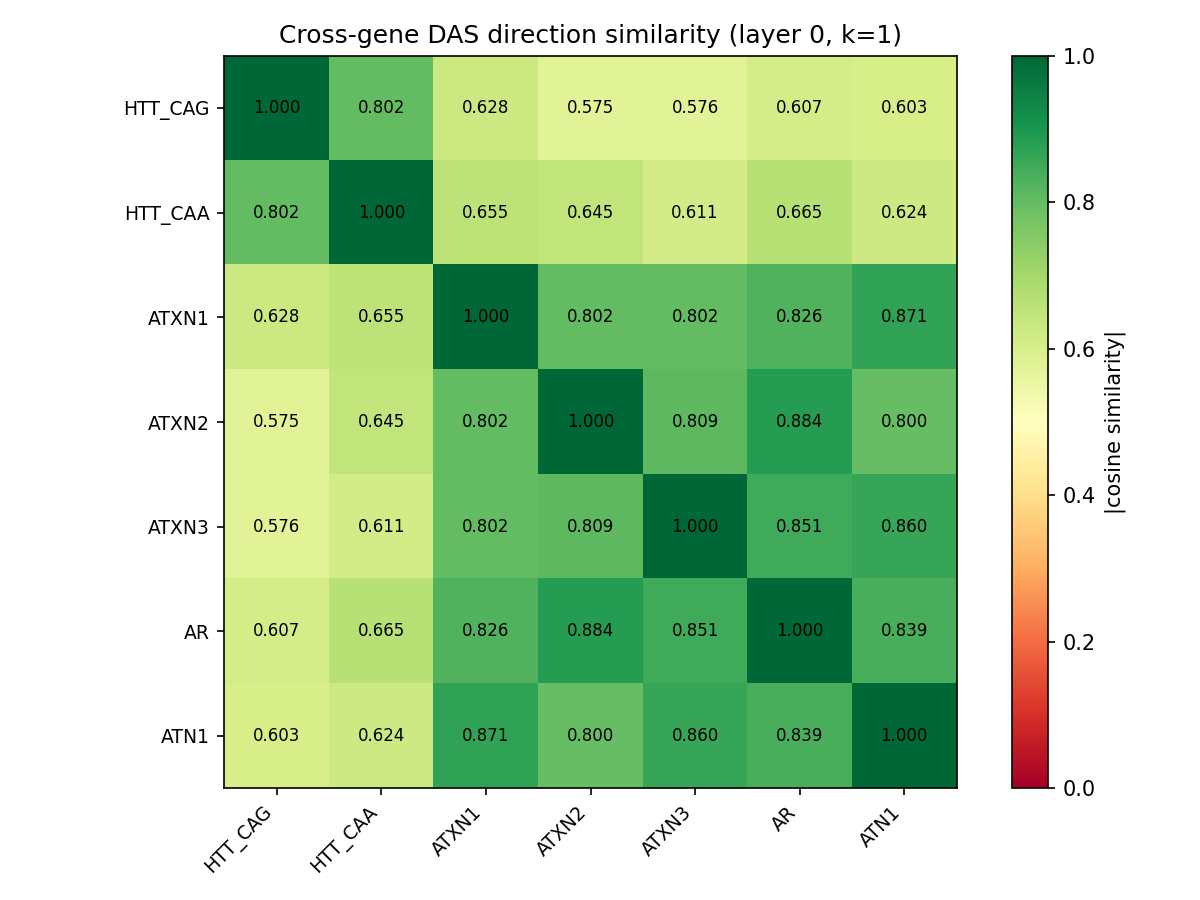
\includegraphics[width=0.7\textwidth]{../figures/cross_gene_directions.png}
\caption{Pairwise $|\cos|$ of DAS directions across 7 conditions.
Two clusters emerge: HTT diverges from the five non-HTT polyglutamine
genes, which share a common encoding subspace. HTT's divergence is
consistent with its unique flanking context (a CCG repeat tract
immediately downstream of the CAG expansion).}
\label{fig:crossgene}
\end{figure}

HTT's divergence is consistent with its distinct flanking context:
HTT exon~1 contains a CCG repeat tract immediately downstream of the
CAG expansion, which the other polyglutamine genes lack. The high
within-cluster similarity among non-HTT genes, despite completely
different flanking sequences, indicates the model reuses a common
repeat-counting mechanism modulated by local sequence context.


%% ────────────────────────────────────────────
\section{Discussion}
\label{sec:discussion}

\subsection{Cross-view independence constrains structural claims}

The strongest empirical result is the statistical independence between
RNA-FM embeddings and ViennaRNA thermodynamic structure. This is a hard
negative: no linear projection of the learned representation recovers
base-pair probability ($|r| < 0.09$), and the subspace overlap is
indistinguishable from random sequences. Any downstream analysis that
assumes RNA-FM embeddings encode secondary structure --- for target
identification, ASO binding prediction, or structural motif
detection --- operates without support from this evidence.

This result does not imply that RNA-FM is uninformative. The model
achieves strong performance on structure prediction benchmarks through
nonlinear readouts (fine-tuned classification heads). The cross-view
analysis tests whether the \emph{linear} subspace structure of
intermediate representations encodes thermodynamic features, which is
the assumption underlying PCA-based and cosine-similarity-based
structural analyses. Nonlinear probing remains a direction for
future work.

\subsection{Metric resolution degrades with representational collapse}

The DI analysis illustrates a general failure mode for directional
metrics on foundation model representations. At layer~6, where 97.9\%
of variance lies in a single principal component, DI is uniform to six
decimal places. The preregistered hypotheses tested at this layer
produce null results that reflect metric blindness rather than absence
of structural sensitivity.

The preregistration specified layer~6 as the primary analysis layer
based on the standard practice of analyzing final-layer
representations. The rank-1 collapse was discovered during the
preregistered analysis, motivating the post-hoc layer~1 re-analysis.
This sequence --- preregister at the conventional layer, discover
collapse, verify at an informative layer --- is itself a finding: the
conventional practice of analyzing final-layer embeddings is
inappropriate for models with extreme late-layer compression.

This failure mode generalizes beyond RNA-FM. Any transformer model
where effective dimensionality drops below $\sim$5 in later layers
will produce uninformative directional metrics at those layers. The
layer-wise effective dimensionality profile should be computed as a
prerequisite to any embedding-based analysis, and the analysis should
target layers where sufficient dimensionality remains.

\subsection{Transportability collapse and drug design}

The Grassmannian transportability result confirms a categorical failure
mode: RNA-FM representations undergo near-complete subspace rotation
($d_g \approx 3.7$, principal angles $> 85^\circ$) for any change in
repeat count, with no gradual degradation or phase transition at the
disease threshold. ASO screening pipelines that rely on embedding
similarity between wild-type and mutant sequences are confounded by
this length-dependent subspace rotation.

The bracket-norm correction identifies which embedding dimensions
encode intensive (per-nucleotide) properties that may be more robust
to repeat-count variation. Drug design should target these dimensions
rather than relying on aggregate subspace geometry.

\subsection{Weight factorization and mechanistic interpretability}

The SVD analysis confirms that RNA-FM's weight matrices have the
low-rank structure required for shared factor bank decomposition. The
$W_Q$ effective rank of 86 in layer~11 (out of 640 dimensions)
implies that $\sim$100--150 learned directions could capture 95\% of
the query-key computation. The high $W_Q$--$W_K$ subspace overlap
(0.81 in layer~3) means these factors would be genuinely shared across
projections, yielding an interpretable decomposition.

\subsection{The encoding--behavior paradox}

The DAS and behavioral invariance results jointly reveal a
paradoxical structure: RNA-FM's embedding layer encodes CAG repeat
count with near-perfect fidelity ($R^2 = 0.992$), yet this information
has zero influence on the model's output (KL $\sim 10^{-6}$). The
encoding is trivial --- it amounts to counting trinucleotide tokens,
as the CAA synonym control confirms. The 12-layer transformer then
progressively destroys this count via MLP-dominated computation in
late layers.

This finding constrains what can be claimed about RNA-FM's internal
representations. Using early-layer embeddings as features for
downstream repeat-count prediction recovers the trivial token-counting
signal. Using late-layer embeddings recovers noise. In neither case
does the $R^2$ value reflect learned biological understanding of
repeat-expansion pathology.

The cross-disease universality ($R^2 > 0.98$ across all six
polyglutamine genes) strengthens this interpretation: the encoding
mechanism is generic to trinucleotide repetitions, independent of
flanking context, codon identity, or biological function. The
two-cluster direction structure (HTT divergent, non-HTT clustered)
adds nuance --- the model's encoding direction is partially
context-specific, living in a $\sim$2D subspace rather than a single
rank-1 direction --- consistent with HTT's unique downstream CCG
repeat tract modulating the embedding geometry.

\subsection{Limitations}

Several limitations qualify these results. RNA-FM was pre-trained
on non-coding RNA; its representations of protein-coding sequences
such as HTT may miss coding-specific structural features. PCA-based
subspace extraction assumes linearity; nonlinear structure would
require manifold learning. The synthetic repeat variants do not
capture somatic mosaicism or epigenetic modifications present in
patient tissue. The DI analysis at layer~1 has $n = 11$ non-WT
variants, limiting statistical power for correlation tests. The CAA
control tests one alternative explanation (length sensitivity) but
does not exhaust all confounds. The weight SVD characterizes the
model's \emph{capacity} for low-rank structure; full
distillation-based factorization requires GPU training.

Two verification checks remain incomplete: a masked-position scope
check (verifying that right-flank positions are included in the
behavioral invariance analysis) and a length-shuffled null (scrambling
the repeat region to distinguish motif-specific from
token-count-specific encoding).

\subsection{Future directions}

Four extensions follow. First, nonlinear cross-view probing ---
training a shallow MLP to predict ViennaRNA base-pair probabilities
from RNA-FM embeddings, testing whether the independence observed at
the linear level persists with nonlinear readouts. Second, full
distillation-based factorization of RNA-FM to extract interpretable
factors, following the pipeline established for
GPT-2~\citep{tower2026fac}. Third, application to additional RNA
therapeutic targets (SARS-CoV-2 frameshifting element, DMD
exon-skipping targets, SMA survival motor neuron) to test
generalizability. Fourth, DAS interchange intervention --- using
the learned rotation to surgically replace the repeat-count
encoding at layer~0 and testing whether downstream representations
and output predictions are affected, providing a causal test of
whether the encoding is functionally inert or merely behaviorally
invisible.


%% ────────────────────────────────────────────
\section{Conclusion}
\label{sec:conclusion}

We applied twelve audits --- six geometric, six causal --- to RNA-FM
representations of CAG repeat regions across all six human
polyglutamine disease genes, under a preregistered analysis protocol.

The geometric audits establish three validity constraints.
RNA-FM embeddings and ViennaRNA thermodynamic predictions are
statistically independent ($|r| < 0.09$, subspace overlap
indistinguishable from shuffled controls). Grassmannian
transportability collapses categorically ($d_g \approx 3.7$) for any
change in repeat count. Direction instability loses resolution on
rank-1-collapsed layers (uniform to six decimal places at layer~6),
recovering genuine signal only at high-dimensionality layers.

The causal probes reveal a paradox. RNA-FM's embedding layer encodes
CAG repeat count with $R^2 = 0.992$ via a single linear direction,
replicated across all six polyglutamine genes ($R^2 > 0.98$) and
confirmed as structure-agnostic by a CAA synonym control ($R^2 =
0.993$). This encoding is progressively destroyed through
MLP-dominated computation (79\% of EAP-IG attribution). By the output
layer, repeat count has zero effect on predictions (100\% top-1
agreement, KL $\sim 10^{-6}$). Cross-gene direction analysis reveals
a two-cluster structure (mean $|\cos| = 0.73$): the encoding lives in
a $\sim$2D subspace, with HTT divergent from the five other genes.

The model represents the clinically relevant variable with high
fidelity but does not compute with it. Using RNA-FM embeddings as
features for repeat-count prediction recovers a trivial
token-counting signal, and any structural claim derived from
these embeddings must be evaluated against these validity constraints.

All code, preregistration records, and data are available at
\url{https://github.com/ElliottTower/causal-rna} under the MIT
license.


%% ────────────────────────────────────────────
\bibliographystyle{plainnat}
% \bibliography{refs}

\begin{thebibliography}{99}

\bibitem[Tower(2026a)]{tower2026bn}
Tower, E.
\newblock Bracket norm: Distinguishing intensive from extensive properties in high-dimensional biomedical feature spaces.
\newblock \emph{Zenodo}, 2026.

\bibitem[Tower(2026b)]{tower2026grass}
Tower, E.
\newblock Grassmannian cohort transfer: Quantifying subspace transportability across biomedical conditions.
\newblock \emph{Zenodo}, 2026.

\bibitem[Tower(2026c)]{tower2026fac}
Tower, E.
\newblock Factorization circuits: Reading transformer circuits from weight decompositions.
\newblock \emph{Zenodo}, 2026.

\bibitem[Chen et al.(2022)]{rnafm}
Chen, J., Hu, Z., Sun, S., Tan, Q., Wang, Y., Yu, Q., Zong, L., Hong, L., Xiao, J., King, I., et al.
\newblock Interpretable RNA foundation model from unannotated data for highly accurate RNA structure and function predictions.
\newblock \emph{arXiv:2204.00300}, 2022.

\bibitem[de~Mezer et al.(2011)]{demezer2011}
de~Mezer, M., Wojciechowska, M., Napierala, M., Sobczak, K., and Krzyzosiak, W.~J.
\newblock Mutant {CAG} repeats of {Huntingtin} transcript fold into hairpins, form nuclear foci and are targets for {RNA} interference.
\newblock \emph{Nucleic Acids Research}, 39(9):3852--3863, 2011.

\bibitem[Devlin et al.(2019)]{devlin2019bert}
Devlin, J., Chang, M.-W., Lee, K., and Toutanova, K.
\newblock {BERT}: Pre-training of deep bidirectional transformers for language understanding.
\newblock In \emph{NAACL-HLT}, 2019.

\bibitem[Edelman et al.(1998)]{edelman1998}
Edelman, A., Arias, T.~A., and Smith, S.~T.
\newblock The geometry of algorithms with orthogonality constraints.
\newblock \emph{SIAM Journal on Matrix Analysis and Applications}, 20(2):303--353, 1998.

\bibitem[MacDonald et al.(1993)]{macdonald1993}
MacDonald, M.~E., Ambrose, C.~M., Duyao, M.~P., et al.
\newblock A novel gene containing a trinucleotide repeat that is expanded and unstable on {Huntington's} disease chromosomes.
\newblock \emph{Cell}, 72(6):971--983, 1993.

\bibitem[Rubinsztein et al.(1996)]{rubinsztein1996}
Rubinsztein, D.~C., Leggo, J., Coles, R., et al.
\newblock Phenotypic characterization of individuals with 30--40 {CAG} repeats in the {Huntington} disease ({HD}) gene reveals {HD} cases with 36 repeats and apparently normal elderly individuals with 36--39 repeats.
\newblock \emph{American Journal of Human Genetics}, 59(1):16, 1996.

\bibitem[Sobczak et al.(2003)]{sobczak2003}
Sobczak, K., de~Mezer, M., Michlewski, G., Krol, J., and Krzyzosiak, W.~J.
\newblock {RNA} structure of trinucleotide repeats associated with human neurological diseases.
\newblock \emph{Nucleic Acids Research}, 31(19):5469--5482, 2003.

\bibitem[Tabrizi et al.(2019)]{tabrizi2019}
Tabrizi, S.~J., Leavitt, B.~R., Landwehrmeyer, G.~B., et al.
\newblock Targeting {Huntingtin} expression in patients with {Huntington's} disease.
\newblock \emph{New England Journal of Medicine}, 380(24):2307--2316, 2019.

\bibitem[Tabrizi et al.(2022)]{tabrizi2022}
Tabrizi, S.~J., Estevez-Fraga, C., van Roon-Mom, W.~M.~C., et al.
\newblock Potential disease-modifying therapies for {Huntington's} disease: lessons learned and future opportunities.
\newblock \emph{The Lancet Neurology}, 21(7):645--658, 2022.

\bibitem[Lorenz et al.(2011)]{lorenz2011viennarna}
Lorenz, R., Bernhart, S.~H., H\"oner zu Siederdissen, C., et al.
\newblock {ViennaRNA} Package 2.0.
\newblock \emph{Algorithms for Molecular Biology}, 6:26, 2011.

\bibitem[Wolf et al.(2020)]{wolf2020transformers}
Wolf, T., Debut, L., Sanh, V., et al.
\newblock Transformers: State-of-the-art natural language processing.
\newblock In \emph{EMNLP: System Demonstrations}, 2020.

\end{thebibliography}

\end{document}
